\chapter{Materials \& Methods} \label{chapter:materials-methods}

% 학위 논문의 결과를 도출하는 데에 사용한 실험 재료와 방법을 타인이 반복 실험 시 동일한 결과를 얻을 수 있을 정도로 자세히 기술한다. 방법에 따라 다음과 같이 부제를 넣어 기술한다.f

% 예)
% 2.1 식물 재료 및 생장 조건
% 2.2 뿌리 관속 조직 관찰
% 2.3 유전자 발현 분석

\section{Space Optimization}

The core idea of \texttt{Petasearch} is actually sacrificing space for fast computation. However, the resources are not limitless. Thus, we would like to keep the cost of space as low as possible while keeping the searching speed high. In this section, we will discuss the space optimization techniques utilized to improve \texttt{Petasearch} prototype.

\subsection{Diff-index Compression} \label{section:diff-index_compression}

As is described in chapter 2, the diff-index created in the k-mer extraction step will store multiple \texttt{USHRT\_MAX} as long as the difference is larger than \texttt{USHRT\_MAX}. This will make any k-mer difference larger than $4 \times \mathtt{USHRT\_MAX} = 262140$ require a larger space to store than the original \texttt{unsigned long} representation. This situation is not uncommon especially when $k$ is large.

Also, in the prototypical implementation, the ID of the source sequence will also be stored multiple times in the ID table. This redundancy is both unnecessary and troublesome. It will increase the size of \texttt{Petasearch} data structures even more than the repeated \texttt{USHRT\_MAX} since the IDs are stored as \texttt{unsigned long} (64-bit integers).


\autoref{fig:k11_space} showed the space consumption of the diff-index created in the k-mer extraction step when $k = 11$. Without optimization, the diff-index (k-mer table) and its corresponding ID table will take up 17 GB of space for a merely 1GB-sized database.

To optimize the size of the diff-index, we devised the bit-squeezing technique to compress the difference between two adjacent k-mers:
For any 64-bit k-mer difference, we continuously fetch 15 bits into a write buffer starting from the least significant bits. We stop the retrieval until we encounter a zero chunk (15 bits of zeros).

To enable the correct decoding of the diff-index during the next phase, the sign bit of the last element in th write is set to \texttt{1} to indicate the end of encoding. Afterwards, we write all the elements in the write buffer to the diff-index. An example encoding process for differecne of value $2039432531946$ is shown in \autoref{fig:bit_squeeze_technique}. For ID table, the optimization is simple: we store the ID of the source sequence only once instead of repeatedly.

Using the bit-squeezing method, it is possible to obtain a maximum of five chunks, making the final space consumption larger than the size of a \texttt{unsigned long} integer. However, such situation only happens when the difference is larger than $\texttt{1UL << 59} = 576460752303423488$, which is extremely rare.

While decoding the compressed diff-index in the process of double-index search, we will reverse the bit-squeezing process through repeatedly retrieving 15 bits from the diff-index table until we encounter the chunk with the sign bit set to \texttt{1}. The decoded difference value will be add to the current k-mer. Moreover, since we do not store redundant IDs, the ID pointer will not be incremented until the end of k-mer decoding. \cref{algorithm:decode_kmer} showed the simplified pseudocode for k-mer decoding.

\begin{algorithm}[htbp]
  \begin{algorithmic}
    \Procedure{DecodeKmer}{$currentKmer$, $currentTargetKmerPtr$, $currentTargetIDPtr$}

    \State $currentDiffIndex \gets 0$\;
    % \State $X \gets x$
    % \State$ $N \gets n$
    \While{$*currentTargetKmerPtr > 0 $}\Comment{This means the sign bit is not 1. }
    \State $currentDiffIndex \gets\ \textsc{Get15Bits}(*currTargetKmerPtr)$
    \State $currentDiffIndex \gets currentDiffIndex \texttt{ << } 15$
    \State $\textsc{Next}(currTargetKmerPtr)$
    \EndWhile
    \State $currentDiffIndex \gets\ \textsc{Get15Bits}(*currTargetKmerPtr)$
    \State $currentKmer \gets currentKmer + currentDiffIndex$
    \State $\textsc{Next}(currTargetKmerPtr)$
    \State $currentTargetIDPtr \gets\ \textsc{Next}(currentTargetIDPtr)$
    \Return $currentKmer$
    \EndProcedure
    \caption{ Pseudocode for the k-mer decoding process} \label{algorithm:decode_kmer}
  \end{algorithmic}
\end{algorithm}

\subsection{Protein Sequence Compression}

For terabyte-size databases, the sequences themselves are also space consuming. To further reduce the size of the databases, we developed the \texttt{ASCII}-sqeezing technique.

Protein sequences are represented by a limited subset of \texttt{ASCII} characters, which are encoded by a single byte. However, as is shown in \autoref{fig:ascii_prot}, we only need 5 bits to represent all the amino acids. Therefore, we can squeeze every three amino acids into one 16-bit \texttt{short}. Similar to the bit-squeezing technique described in \cref{section:diff-index_compression}, we also use the sign bit to indicated the end of the compressed protein sequence. \autoref{fig:prot_seq_compress} showed an example compression process for glutathione (GSH). The \texttt{ASCII}-squeezing technique is expected to produce a sqeuence database about $85\%$ of the original size.


\begin{figpage}
  \begin{figure}
    \centering
    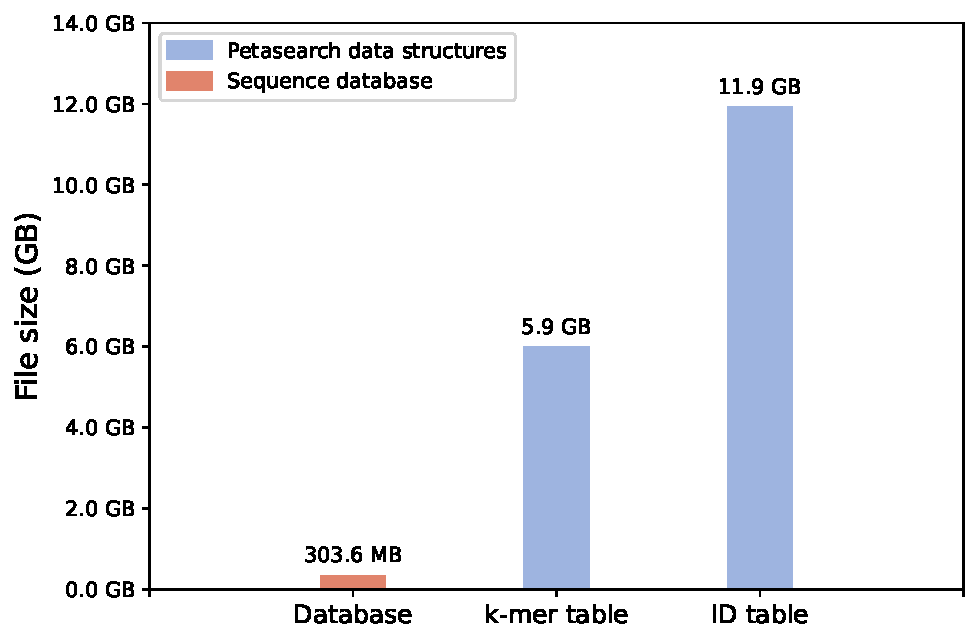
\includegraphics[width=.65\textwidth]{images/k11_space_consumption.pdf}
    \captionof{figure}{Visualizaiton of k-mer table and ID table sizes when $k = 11$. The database is the \texttt{UniProtKB/Swiss-Prot} database obtained through \texttt{mmseqs databases UniProtKB/Swiss-Prot swissprot tmp} command. Without optimization, the sizes of \texttt{petasearch} data structures are 6.46 times and 12.92 times larger than the sequence database.}
    \label{fig:k11_space}
    \bigskip
    \centering
    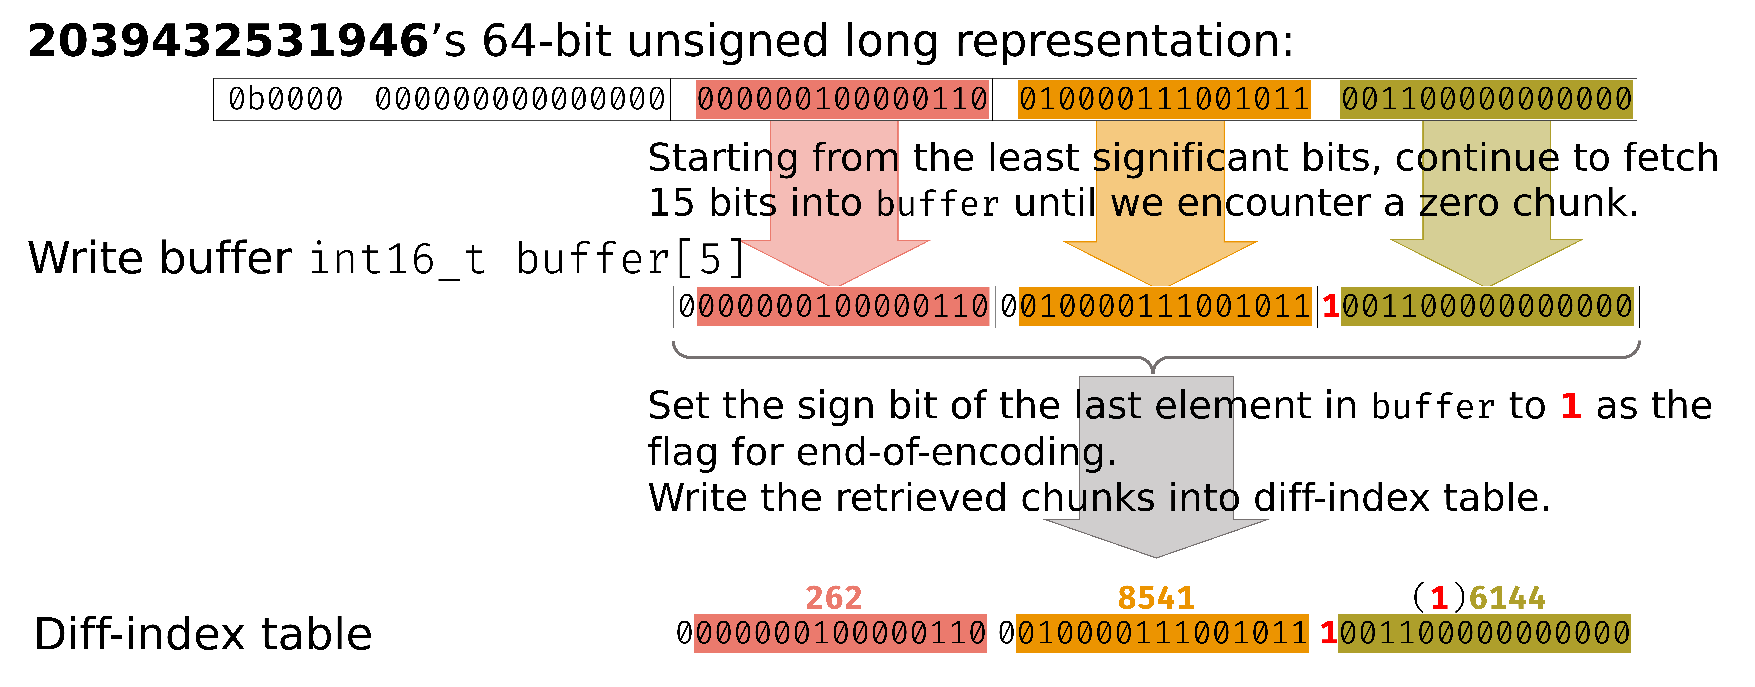
\includegraphics[width=\textwidth]{images/bit_squeezing_technique.pdf}
    \captionof{figure}{The example decoding process of difference index $2039432531946$. We first retrieve 15-bit chunks starting from the least significant bits and store them into a write buffer in the reverse order until we encounter a zero chunk. For $2039432531946$, its highest non-zero bit is $39$, which means that we need three 16-bit \texttt{short} to store it.}
    \label{fig:bit_squeeze_technique}
  \end{figure}
\end{figpage}

\section{Speed Optimization}

Speed is the first and foremost concern of \texttt{Petasearch}. The speed of \texttt{Petaserch} prototype is already fast, but did not make it stand out too much from its competitors. In this section, we will introduce several techniques to further boost the speed of \texttt{Petasearch}.

\subsection{IO Performance Optimization}

In the prototypical \texttt{Petasearch} implementation, \texttt{mmap} was selected for reading \texttt{Petasearch} data structures stored on NVMe SSDs. However, \texttt{mmap} does not scale well with the increase in threads (\cite{papagiannis2020optimizing}) and thus cannot saturate the full throughput of NVMe SSDs. To find the IO tool with the best performance, we conducted a benchmarking study on the performance of various IO tools using FIO benchmark software (\cite{AxboeFlexibleIOTester2022}). For synced IO tools, we benchmarked \texttt{pread} using different flags and \texttt{mmap}. For async IO tools, we benchmarked \texttt{libaio} and \texttt{posix\_aio}.

The benchmarking results are visualized in \autoref{fig:fio_benchmark}. It is clear that \texttt{libaio} performs the best. I is able to saturate the full 3.5 GB/s linear read bandwidth of NVMe SSDs. The other two tools, \texttt{posix\_aio} and \texttt{pread} with \texttt{O\_DIRECT} (\texttt{ioengine = psync} in FIO) have roughly the same performance, with bandwidth around 3.3 GB/s. Unfortunately, \texttt{mmap} has the worst performance, with only about 1.5 GB/s at maximum. The performance even fell to 0.25 GB/s when it scaled to 20 threads. Since \texttt{mmap} is a synced IO module, adopting another synced IO module will require almost no change in control logic. Considering both the performance and difficulty of refactoring, we chose to use \texttt{pread} with \texttt{O\_DIRECT} in place of \texttt{mmap}.

The implementation of \texttt{pread} with \texttt{O\_DIRECT} is rather simple: we simply create a read buffer according to the currently available memory size, open the k-mer diff-index file with \texttt{O\_DIRECT} flag, and then read in parallel using \texttt{pread} continuously untill \texttt{EOF} (end of file).

\subsection{Simplified Database Index}

In \texttt{Pteasearch} prototype, the sequence database format is the same as that of \texttt{MMseqs}, which has many functions uses a complexed index structure. Such complexity is unnecessary for \texttt{Petasearch}. Hence, we simplified the index, only preservingthe offset of the corresponding entry in the sequence database. It is expected to reduce the IO time.

\begin{figpage}
  \thispagestyle{fancy}
  \begin{figure}[htbp]
    \centering
    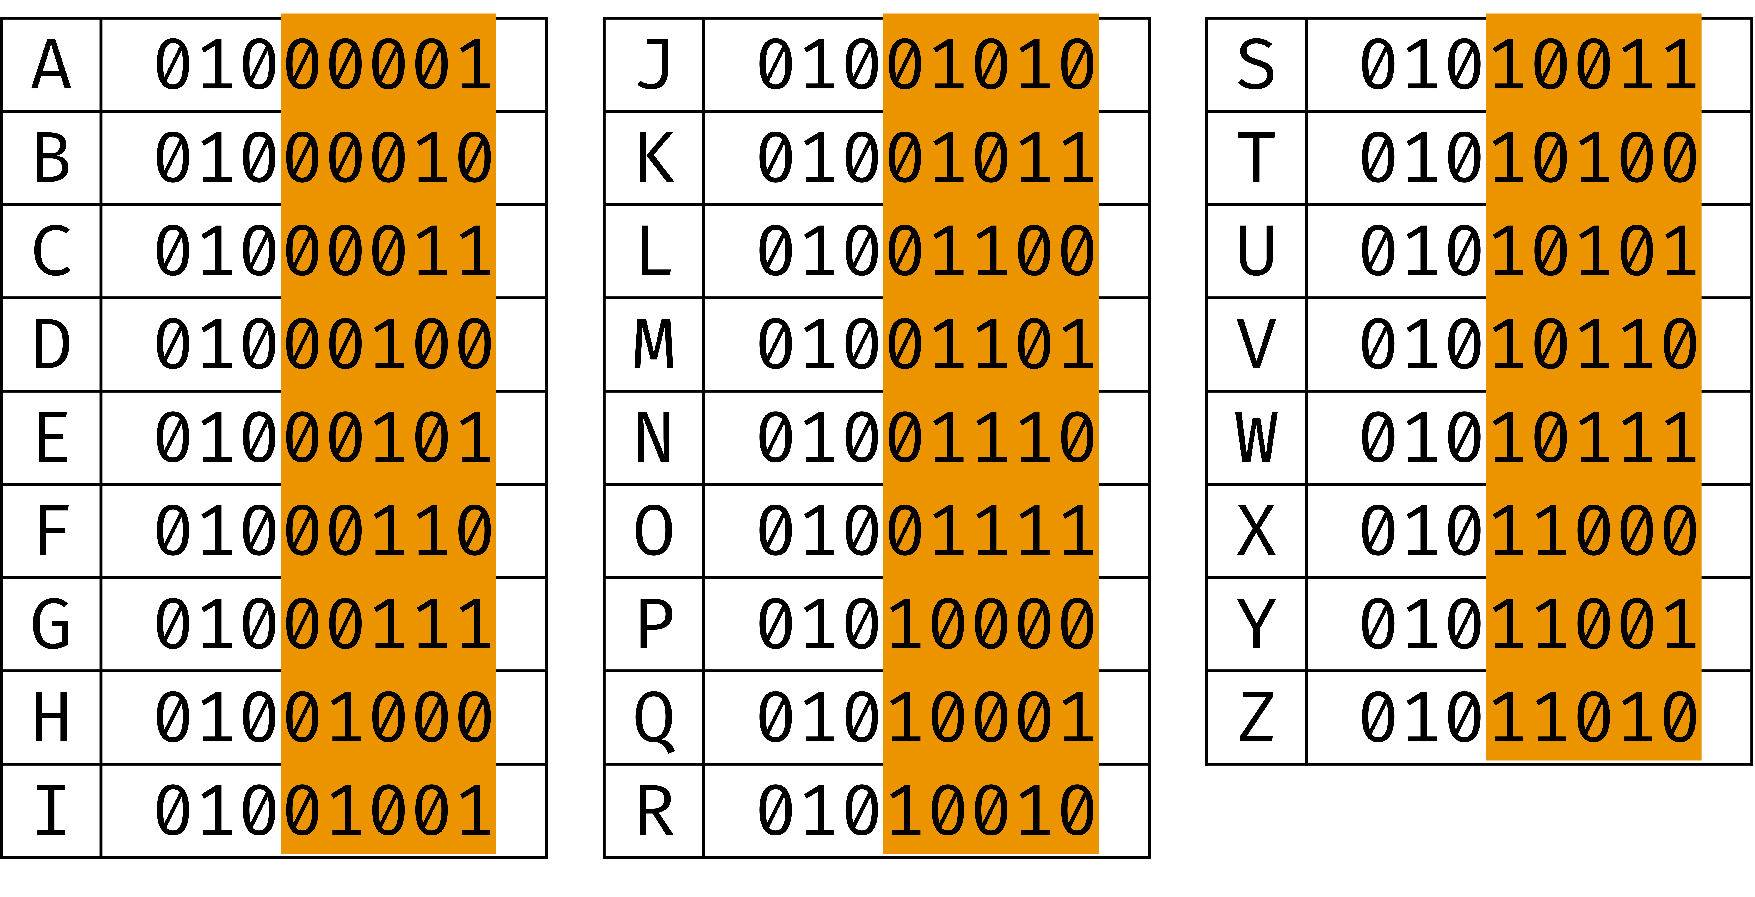
\includegraphics[width=.6\textwidth]{images/ASCII_prot.pdf}
    \caption{Part of the ASCII table, showing the bit representation of \texttt{A} to \texttt{Z} with the last 5 bits highlighted. It can be clearly seen that for \texttt{A} to \texttt{Z} in the English alphabet, we can represent them using only 5 bits instead of a whole byte (8 bits).}
    \label{fig:ascii_prot}
    \bigskip
    \centering
    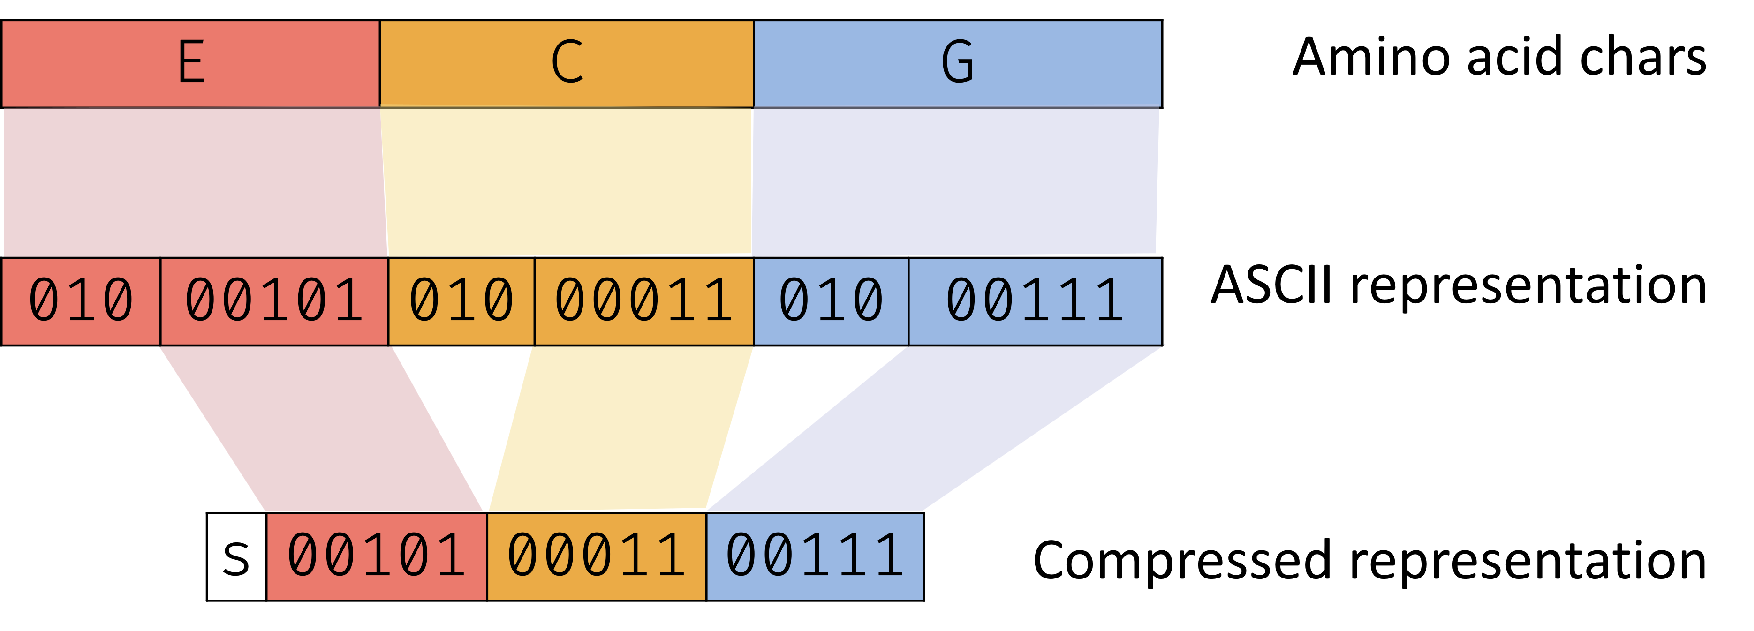
\includegraphics[width=.9\textwidth]{images/prot_seq_compress.pdf}
    \caption{The example compression of short peptide glutathione (GSH). GSH consists of only three amino acids: glutamate (E), cysteine (C), and glycine (G). We simply fetch the least significant 5 bits of each amino acid \texttt{char} and store them into a single 16-bit \texttt{short}.}
    \label{fig:prot_seq_compress}
    \bigskip
    \centering
    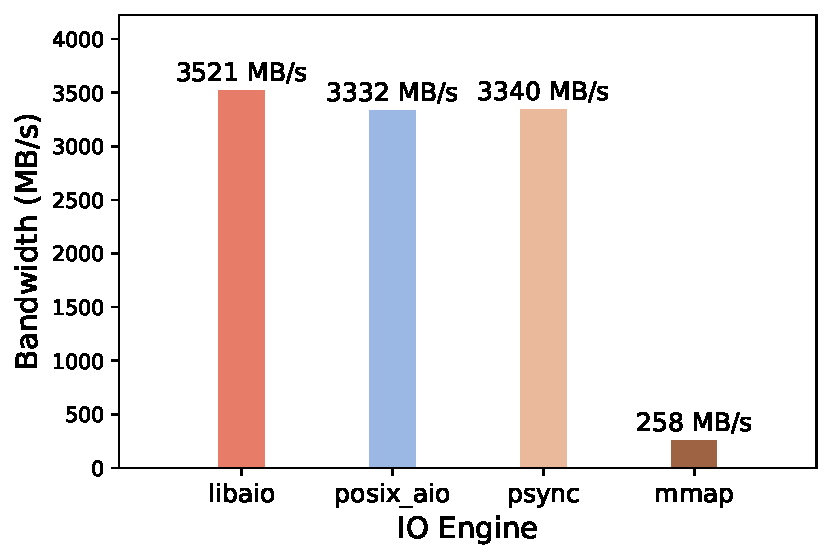
\includegraphics[width=.65\textwidth]{images/fio_benchmark.pdf}
    \caption{Benchmarking results of various IO tools using FIO benchmark software. The benchmark setting is imitating a parallel read from 20 NVMe SSDs. A total of 20 threads were created, each one responsible of reading a 50 GB file stored on one NVMe SSD. The bandwidth is the average reading bandwidth per SSD. The IO engine \texttt{psync} is equivalent to opening a file handle with \texttt{O\_DIRECT} and reading from the handle using \texttt{pread}.}
    \label{fig:fio_benchmark}
  \end{figure}
\end{figpage}

\subsection{Fast Third-Party Libraries}

We integrated several fast thrid-party libraries to replace the slow implementaions in \texttt{Petaserch} prototype. The fast parallel in-place sorting algorithm $IPS^4o$ (\cite{axtmann2017place}) was integrated to replace the slow \texttt{std::sort}. The banded Smith-Waterman-Gotoh aligner \texttt{block-aligner} (\cite{liu2021block}) was used to allow fast pairwise alignment in the third phase.

\section{Sensitivity Improvement}

The k-mer matching mechanism limits \texttt{Petasearch}'s ability of finding homologs with low sequence identity. To improve \texttt{Petasearch}'s performance at lower sequence identity, we made \texttt{Petasearch} able to perform profile search by allowing profile databases as inputs.

Profile search is using a "sequence profile" generated from multiple sequence alignment (MSA) results as the querying input (\cite{steinegger2019hh}). The profile Hidden Markov Model (HMM) provides position-specific aminoaid indel and substitution penalties (\cite{steinegger2019hh}), which significantly increase the searching sensitivity. The most sensitive searching tools such as \texttt{HMMER} (\cite{eddy2009new}, \cite{eddy2011accelerated}), \texttt{HHblits} (\cite{remmert2012hhblits}) and \texttt{HH-suite3} (\cite{steinegger2019hh}) all use the profile search mechanism. Thus, enabling \texttt{Petaserch} to perform profile search is expected to improve its sensitivity at low sequence identity.
